\documentclass{standalone}

\usepackage{../core}

\def\ystep{0.137255in}
\def\yoff{0.017in}
\def\yg{17.9}
\def\xgstep{0.525}

\begin{document}
\begin{tikzpicture}[
  C/.style={circle,
            align=center,
            draw=darkcolor,
            line width=0.7pt,
            text=textcolor,
            inner sep=2pt,
            minimum height=2.5em
            },
  G/.style={anchor=south,
            text=textcolor,
            inner sep=0pt
            },
  M/.style={anchor=south west,
            draw=darkcolor,
            thin,
            inner sep=1pt
            },
  N/.style={text=textcolor,
            anchor=south east,
            inner sep=0pt,
            xshift=-2.43in
            }
]

\node[C] at (0.68,19.2) {\large \strut $\*u$};
\node[C] at (4.58,19.2) {\large $\,\*W$};
\node[C] at (10.4,19.2) {\large $\,\*V$};

\node[M] at (0,0) {
\includegraphics[height=7in]{mat_aml_u.png}};
\node[M] at (1.9,0) {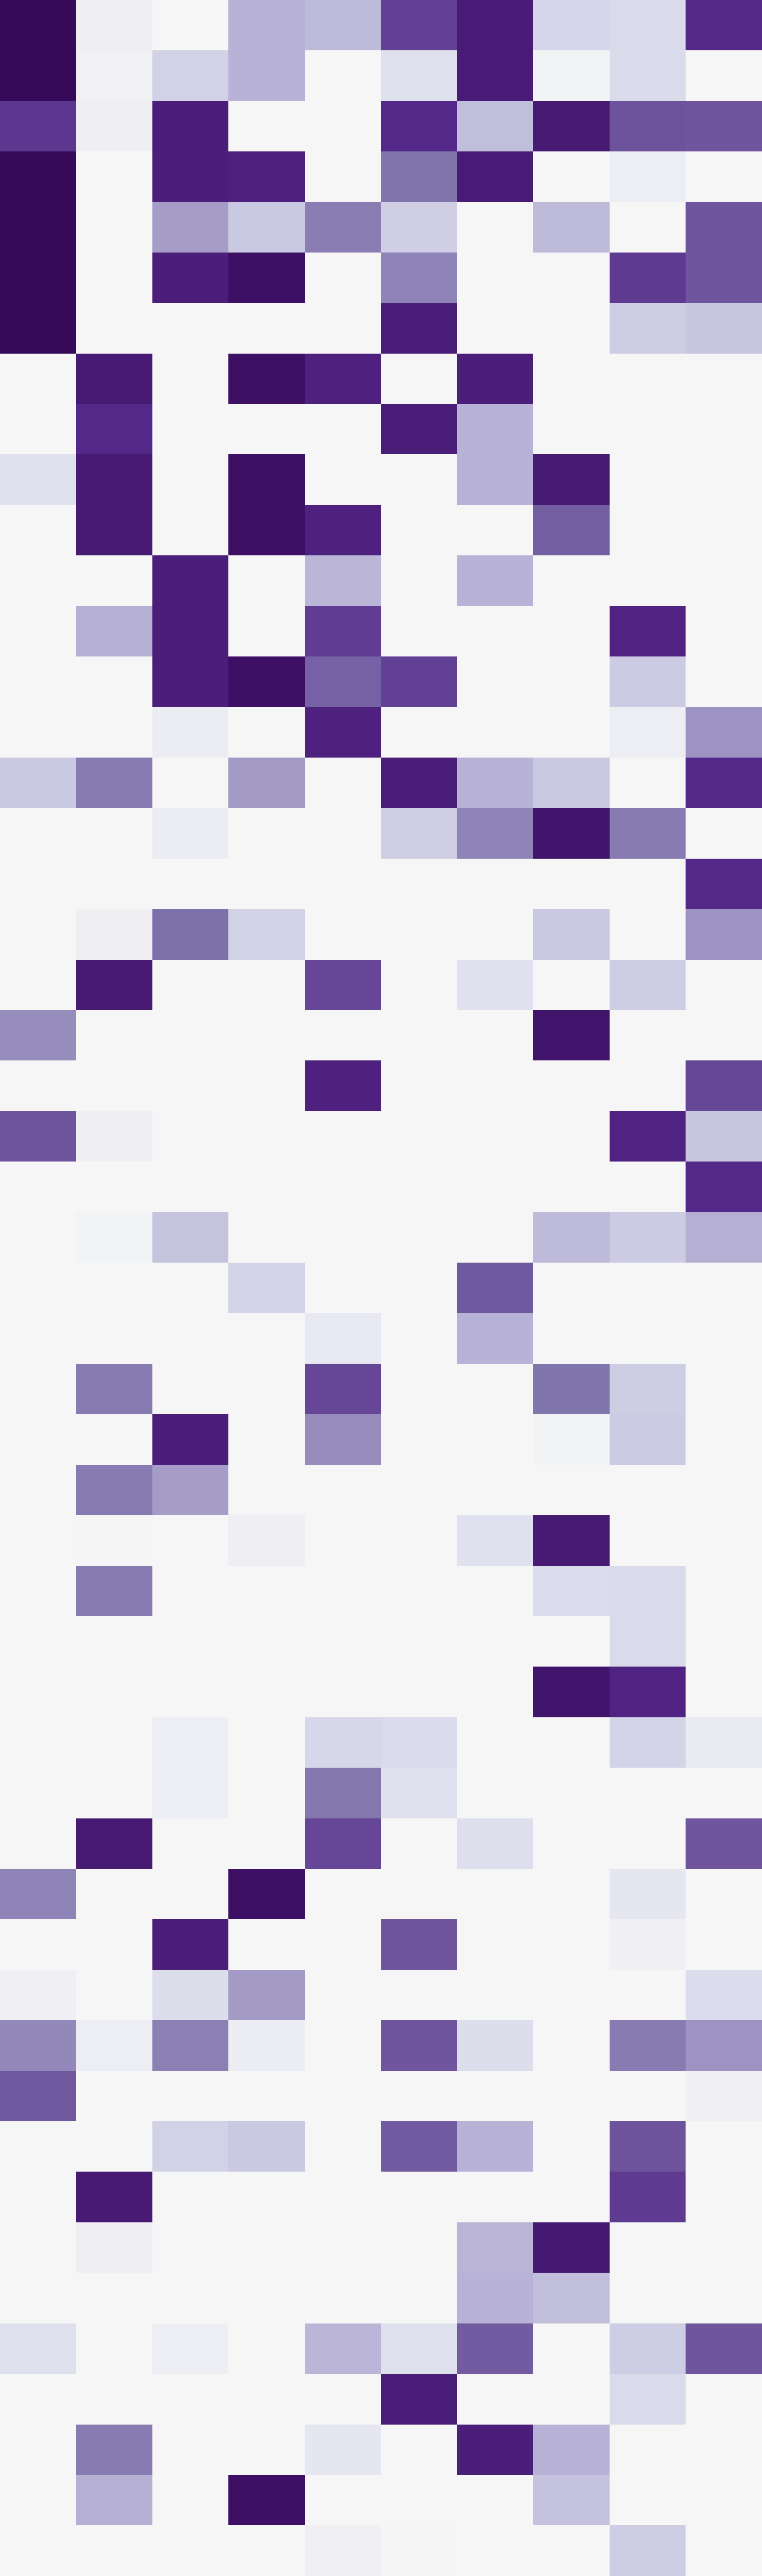
\includegraphics[height=7in]{mat_aml_w.png}};
\node[M] at (7.75,0) {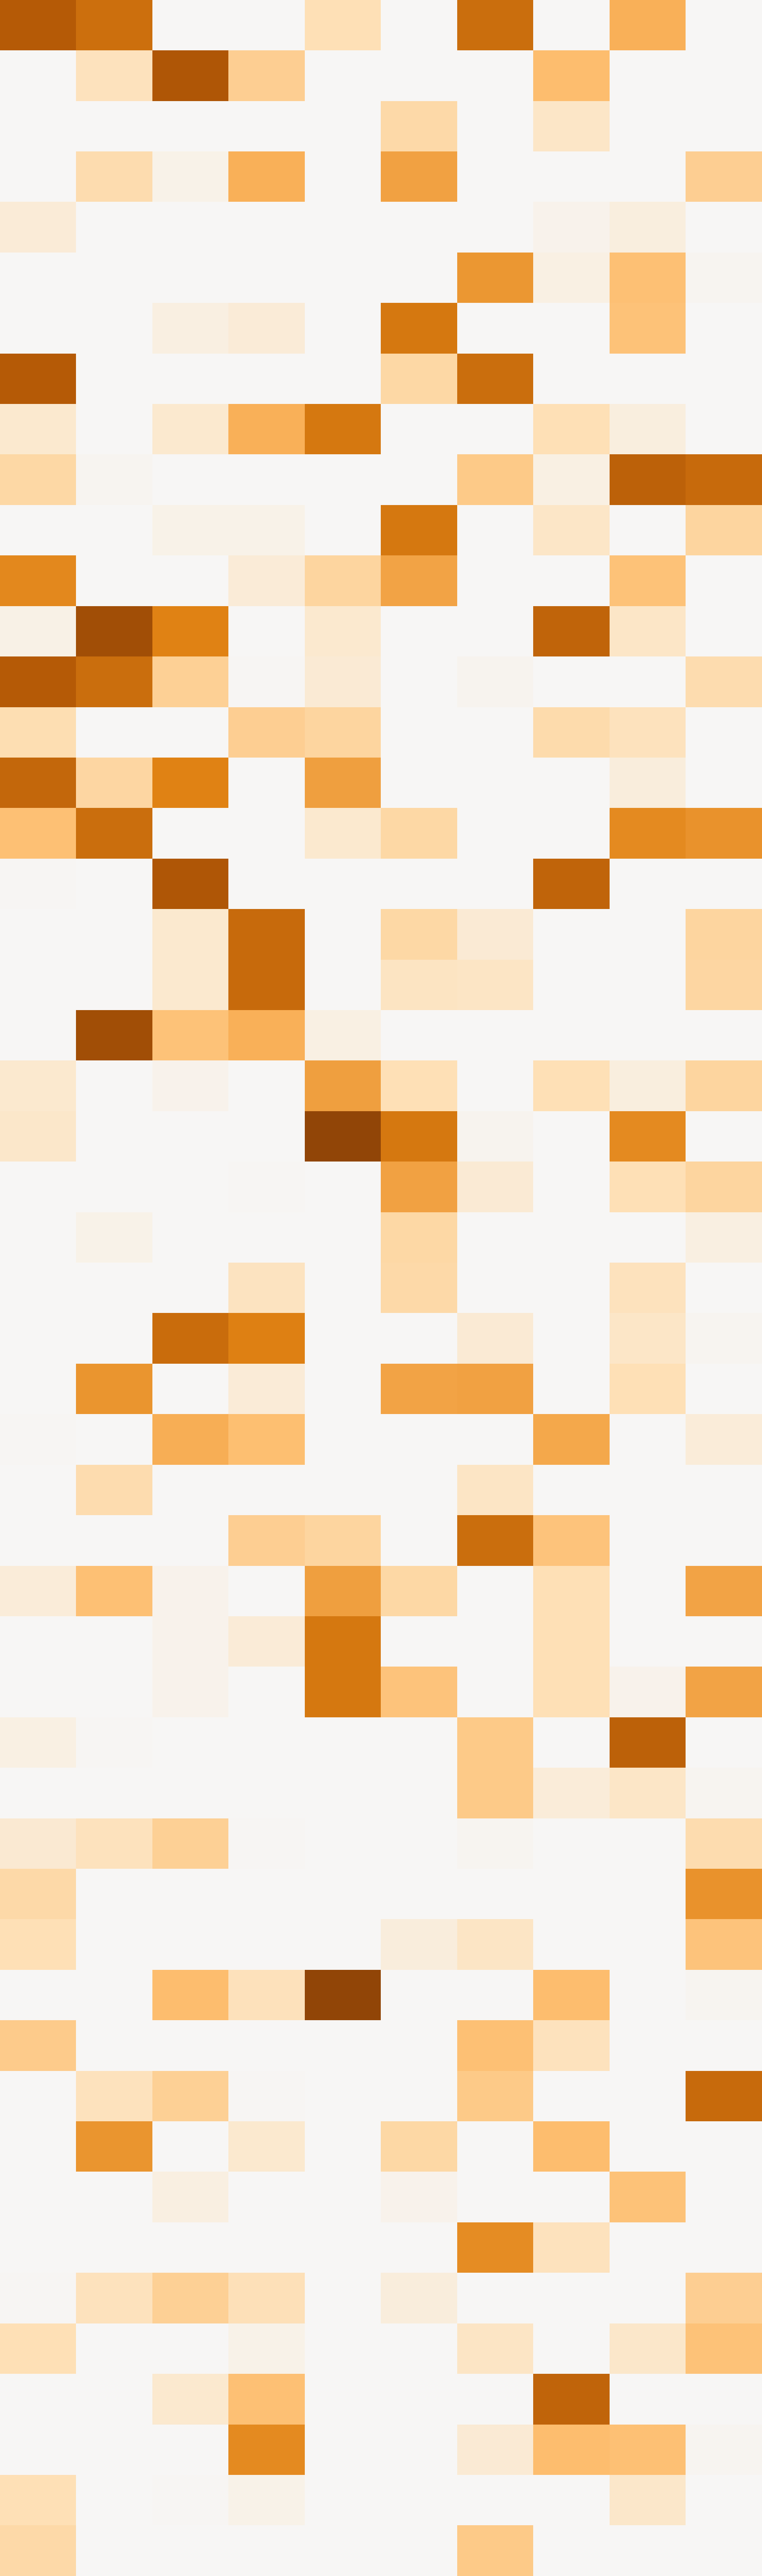
\includegraphics[height=7in]{mat_aml_v.png}};

\node[N,yshift=50*\ystep-\yoff] at (current page.south) {\sffamily \strut NPM1};
\node[N,yshift=49*\ystep-\yoff] at (current page.south) {\sffamily \strut RUNX1};
\node[N,yshift=48*\ystep-\yoff] at (current page.south) {\sffamily \strut PML-RARα};
\node[N,yshift=47*\ystep-\yoff] at (current page.south) {\sffamily \strut TP53};
\node[N,yshift=46*\ystep-\yoff] at (current page.south) {\sffamily \strut MLL-fusions};
\node[N,yshift=45*\ystep-\yoff] at (current page.south) {\sffamily \strut MYH11-CBFβ};
\node[N,yshift=44*\ystep-\yoff] at (current page.south) {\sffamily \strut RUNX1-RUNX1T1};
\node[N,yshift=43*\ystep-\yoff] at (current page.south) {\sffamily \strut FLT3};
\node[N,yshift=42*\ystep-\yoff] at (current page.south) {\sffamily \strut Ser./Thr. kinases};
\node[N,yshift=41*\ystep-\yoff] at (current page.south) {\sffamily \strut NRAS/KRAS};
\node[N,yshift=40*\ystep-\yoff] at (current page.south) {\sffamily \strut Tyr. kinases};
\node[N,yshift=39*\ystep-\yoff] at (current page.south) {\sffamily \strut Cohesin comp.};
\node[N,yshift=38*\ystep-\yoff] at (current page.south) {\sffamily \strut IDH2};
\node[N,yshift=37*\ystep-\yoff] at (current page.south) {\sffamily \strut IDH1};
\node[N,yshift=36*\ystep-\yoff] at (current page.south) {\sffamily \strut Spliceosome};
\node[N,yshift=35*\ystep-\yoff] at (current page.south) {\sffamily \strut MLL-PTD};
\node[N,yshift=34*\ystep-\yoff] at (current page.south) {\sffamily \strut DNMT3A};
\node[N,yshift=33*\ystep-\yoff] at (current page.south) {\sffamily \strut ASXL1};
\node[N,yshift=32*\ystep-\yoff] at (current page.south) {\sffamily \strut Epig. mods};
\node[N,yshift=31*\ystep-\yoff] at (current page.south) {\sffamily \strut NF1};
\node[N,yshift=30*\ystep-\yoff] at (current page.south) {\sffamily \strut MIR142};
\node[N,yshift=29*\ystep-\yoff] at (current page.south) {\sffamily \strut PHACTR1};
\node[N,yshift=28*\ystep-\yoff] at (current page.south) {\sffamily \strut TET2};
\node[N,yshift=27*\ystep-\yoff] at (current page.south) {\sffamily \strut CROCC};
\node[N,yshift=26*\ystep-\yoff] at (current page.south) {\sffamily \strut CACNA1B};
\node[N,yshift=25*\ystep-\yoff] at (current page.south) {\sffamily \strut CACNA1E};
\node[N,yshift=24*\ystep-\yoff] at (current page.south) {\sffamily \strut PLCE1};
\node[N,yshift=23*\ystep-\yoff] at (current page.south) {\sffamily \strut PTPs};
\node[N,yshift=22*\ystep-\yoff] at (current page.south) {\sffamily \strut DIS3};
\node[N,yshift=21*\ystep-\yoff] at (current page.south) {\sffamily \strut MT-CO2};
\node[N,yshift=20*\ystep-\yoff] at (current page.south) {\sffamily \strut WT1};
\node[N,yshift=19*\ystep-\yoff] at (current page.south) {\sffamily \strut MT-CYB};
\node[N,yshift=18*\ystep-\yoff] at (current page.south) {\sffamily \strut GRIK2};
\node[N,yshift=17*\ystep-\yoff] at (current page.south) {\sffamily \strut SPEN};
\node[N,yshift=16*\ystep-\yoff] at (current page.south) {\sffamily \strut COL12A1};
\node[N,yshift=15*\ystep-\yoff] at (current page.south) {\sffamily \strut FCGBP};
\node[N,yshift=14*\ystep-\yoff] at (current page.south) {\sffamily \strut BCR-ABL1};
\node[N,yshift=13*\ystep-\yoff] at (current page.south) {\sffamily \strut Myeloid tfs.};
\node[N,yshift=12*\ystep-\yoff] at (current page.south) {\sffamily \strut MT-RNR1};
\node[N,yshift=11*\ystep-\yoff] at (current page.south) {\sffamily \strut DNAH9};
\node[N,yshift=10*\ystep-\yoff] at (current page.south) {\sffamily \strut NUP98-NSD1};
\node[N,yshift=9*\ystep-\yoff] at (current page.south) {\sffamily \strut EZH2};
\node[N,yshift=8*\ystep-\yoff] at (current page.south) {\sffamily \strut PHF6};
\node[N,yshift=7*\ystep-\yoff] at (current page.south) {\sffamily \strut KDM6A};
\node[N,yshift=6*\ystep-\yoff] at (current page.south) {\sffamily \strut GPR128-TFG};
\node[N,yshift=5*\ystep-\yoff] at (current page.south) {\sffamily \strut MT-ND5};
\node[N,yshift=4*\ystep-\yoff] at (current page.south) {\sffamily \strut CEBPA};
\node[N,yshift=3*\ystep-\yoff] at (current page.south) {\sffamily \strut MT-CO3};
\node[N,yshift=2*\ystep-\yoff] at (current page.south) {\sffamily \strut KIT};
\node[N,yshift=1*\ystep-\yoff] at (current page.south) {\sffamily \strut GBP4};
\node[N,yshift=0*\ystep-\yoff] at (current page.south) {\sffamily \strut FAM5C};


\node[M] at (0,-0.8) {
\includegraphics[width=0.52in,height=0.115in]{cbar_aml_u.png}};
\node[M] at (1.9,-0.8) {
\includegraphics[width=2.08in]{cbar_aml_w.png}};
\node[M] at (7.75,-0.8) {
\includegraphics[width=2.08in]{cbar_aml_v.png}};

\node[text=textcolor] at (0,-1.1) {\sffamily -6};
\node[text=textcolor] at (1.37,-1.1) {\sffamily 1};

\node[text=textcolor] at (1.94,-1.1) {\sffamily 0};
\node[text=textcolor] at (7.25,-1.1) {\sffamily 2};

\node[text=textcolor] at (7.79,-1.1) {\sffamily 0};
\node[text=textcolor] at (13.1,-1.1) {\sffamily 3};

\end{tikzpicture}
\end{document}